% -*- coding: utf-8 -*-
\newpage
\section{Zero Nuclear Contribution}\label{zero_nuclear_contribution}

The following graphs illustrate all possible subsets that can occur within a
given system, each of which may be regarded as part of a larger set. In the
particular cases shown here, all atoms within the subset carry zero charge.  If
this condition holds, then the inclusion of any additional atom into the subset
will also yield zero charge, as the added atom will necessarily be bonded to an
entire subsystem already carrying zero charge. In practice, a nuclear
contribution of the dipole moment of exactly zero implies all atoms have zero
charge, a situation that is highly improbable in most chemical systems.

\begin{figure}[ht]
  \centering
  \scalebox{0.5}{\begingroup
\setmainfont{DejaVu Sans}

\resizebox{\linewidth}{!}{%
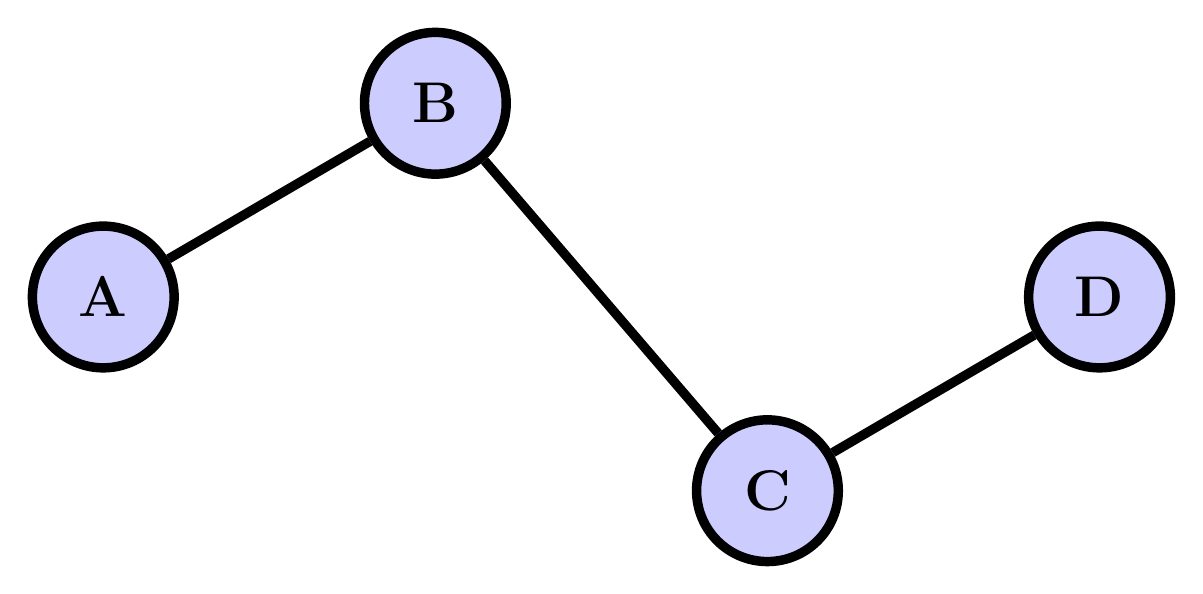
\begin{tikzpicture}
  \tikzset{
    mynode/.style={
      circle,
      draw=black,
      fill=blue!20,
      line width=1.2mm,
      minimum size=18mm,
      font=\bfseries\fontsize{20}{20}\selectfont,
      text centered
    }
  }

  \node[mynode] (A) at (0pt, 0pt) {A};
  \node[mynode] (B) at (120pt, 70pt) {B};
  \node[mynode] (C) at (240pt, -70pt) {C};
  \node[mynode] (D) at (360pt, 0pt) {D};

  \draw[line width=1.2mm] (A) -- (B);
  \draw[line width=1.2mm] (B) -- (C);
  \draw[line width=1.2mm] (C) -- (D);
\end{tikzpicture}%
}
\endgroup

}
  \caption{System of atoms bonded in a chain.}
  \label{first_case}
\end{figure}

\begin{align}
\text{trivial case:} \nonumber\\
  if\: q(\mathrm{A}|\mathrm{B}) &= 0 \nonumber\\
    & \implies q(\mathrm{A}) = q(\mathrm{B}) = 0
\end{align}

\newpage

\begin{figure}[ht]
  \centering
  \scalebox{.3}{\begingroup
\setmainfont{DejaVu Sans}

\resizebox{\linewidth}{!}{%
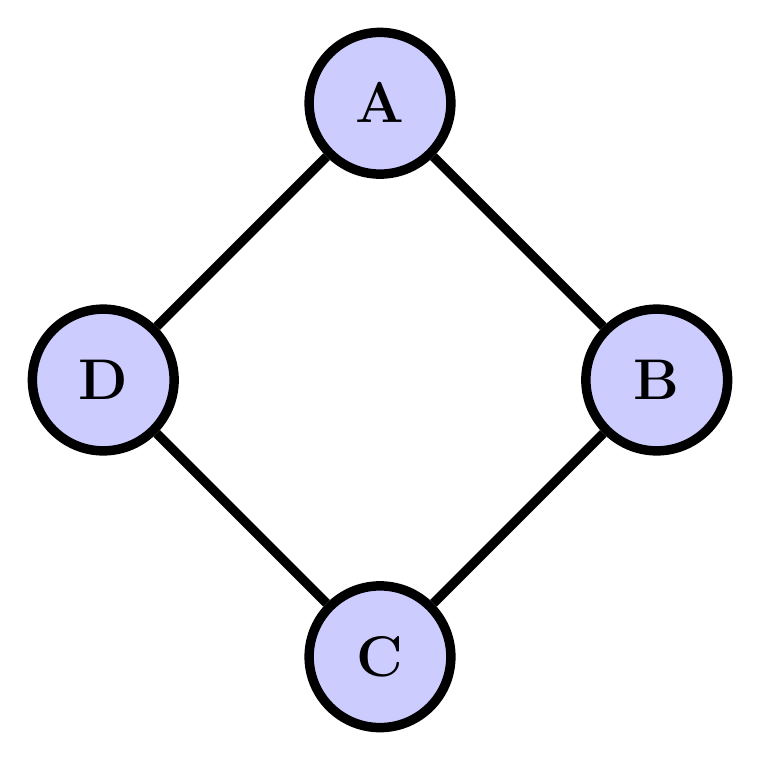
\begin{tikzpicture}
  \tikzset{
    mynode/.style={
      circle,
      draw=black,
      fill=blue!20,
      line width=1.2mm,
      minimum size=18mm,
      font=\bfseries\fontsize{20}{20}\selectfont,
      text centered
    }
  }

  \node[mynode] (A) at (0pt, 100pt) {A};
  \node[mynode] (B) at (100pt, 0pt) {B};
  \node[mynode] (C) at (0pt, -100pt) {C};
  \node[mynode] (D) at (-100pt, 0pt) {D};

  \draw[line width=1.2mm] (A) -- (B);
  \draw[line width=1.2mm] (B) -- (C);
  \draw[line width=1.2mm] (C) -- (D);
  \draw[line width=1.2mm] (D) -- (A);
\end{tikzpicture}%
}
\endgroup

}
  \caption{System of atoms bonded in a ring.}
  \label{second_case}
\end{figure}

\begin{align}
    if\: q(\mathrm{A}|\mathrm{B}) &= 0 \nonumber\\
      & \implies q(\mathrm{A}) = q(\mathrm{A}|\mathrm{D}) \nonumber \\
      & \implies q(\mathrm{B}) = q(\mathrm{B}|\mathrm{C}) \nonumber \\
      & \implies q(\mathrm{C}) = q(\mathrm{C}|\mathrm{B}) + q(\mathrm{C}|\mathrm{D}) \nonumber \\
      & \implies q(\mathrm{A}|\mathrm{B}) + q(\mathrm{B}|\mathrm{C}) + q(\mathrm{C}|\mathrm{D}) + q(\mathrm{D}|\mathrm{A}) = 0 \nonumber \\
      & \implies q(\mathrm{B}) + q(\mathrm{C}) - q(\mathrm{C}|\mathrm{B}) - q(\mathrm{A}) = 0 \nonumber \\
      & \implies q(\mathrm{D}) = q(\mathrm{D}|\mathrm{A}) + q(\mathrm{D}|\mathrm{C}) \nonumber \\
      & \implies q(\mathrm{A}) = -q(\mathrm{D}) + q(\mathrm{D}|\mathrm{C}) \nonumber \\
      & \implies 2q(\mathrm{B}) + q(\mathrm{C}) = q(\mathrm{A}) \nonumber \\
      & \implies q(\mathrm{A}) = -q(\mathrm{D}) + q(\mathrm{D}|\mathrm{C}) \nonumber \\
      & \implies q(\mathrm{A}) = q(\mathrm{B}) + q(\mathrm{C}) - q(\mathrm{C}|\mathrm{B}) \nonumber \\
      &\therefore q(\mathrm{B}) = -q(\mathrm{C}|\mathrm{B}) = -q(\mathrm{B})
\end{align}

\newpage

\begin{figure}[ht]
  \centering
  \scalebox{.4}{\begingroup
\setmainfont{DejaVu Sans}

\resizebox{\linewidth}{!}{%
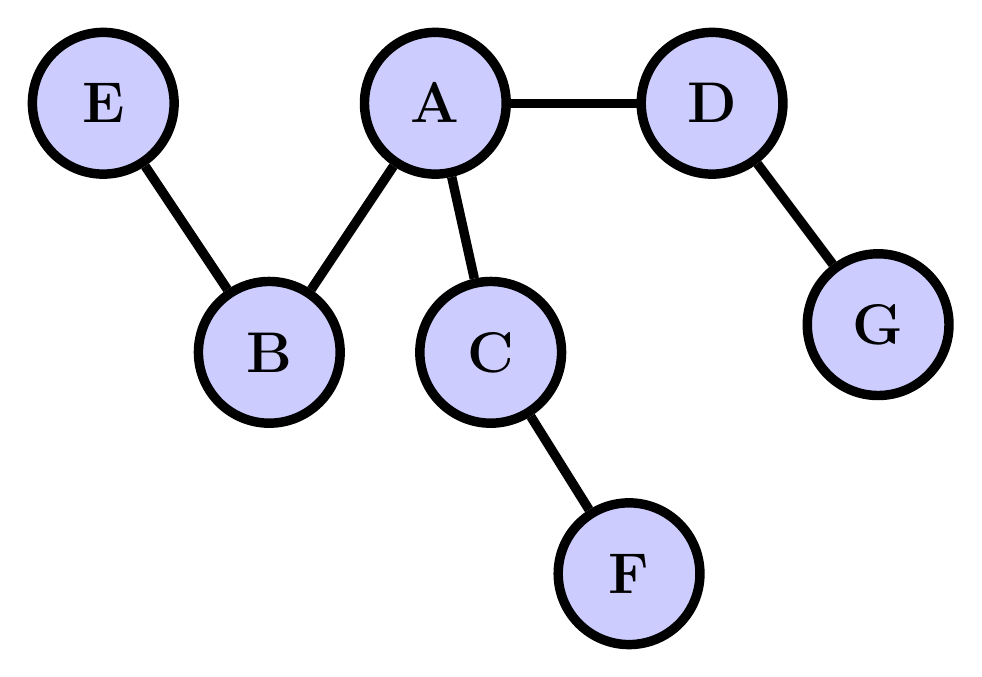
\begin{tikzpicture}
  \tikzset{
    mynode/.style={
      circle,
      draw=black,
      fill=blue!20,
      line width=1.2mm,
      minimum size=18mm,
      font=\bfseries\fontsize{20}{20}\selectfont,
      text centered
    }
  }

  \node[mynode] (A) at (0pt, 150pt) {A};
  \node[mynode] (B) at (-60pt, 60pt) {B};
  \node[mynode] (C) at (20pt, 60pt) {C};
  \node[mynode] (D) at (100pt, 150pt) {D};
  \node[mynode] (E) at (-120pt, 150pt) {E};
  \node[mynode] (F) at (70pt, -20pt) {F};
  \node[mynode] (G) at (160pt, 70pt) {G};

  \draw[line width=1.2mm] (A) -- (B);
  \draw[line width=1.2mm] (A) -- (C);
  \draw[line width=1.2mm] (A) -- (D);
  \draw[line width=1.2mm] (B) -- (E);
  \draw[line width=1.2mm] (C) -- (F);
  \draw[line width=1.2mm] (D) -- (G);
\end{tikzpicture}%
}
\endgroup

}
  \caption{System of atoms bonded in a branched chain.}
  \label{third_case}
\end{figure}

\begin{align}
  if\, q(\mathrm{A}|\mathrm{B}) &= 0 \nonumber \\
    & \implies q(\mathrm{B}) = q(\mathrm{E}) \nonumber \\
    & \implies q(\mathrm{A}) = q(\mathrm{A}|\mathrm{C}) + q(\mathrm{A}|\mathrm{D}) \nonumber \\
    & \implies q(\mathrm{D}) = q(\mathrm{D}|\mathrm{G}) + q(\mathrm{D}|\mathrm{A}) \nonumber \\
    & \implies q(\mathrm{G}) = q(\mathrm{G}|\mathrm{D}) \nonumber \\
    & \implies q(\mathrm{D}) = -q(\mathrm{G}) -q(\mathrm{A}) + q(\mathrm{A}|\mathrm{C}) \nonumber \\
    & \implies q(\mathrm{A}) = q(\mathrm{A}|\mathrm{C}) + q(\mathrm{A}|\mathrm{D}) + q(\mathrm{A}|\mathrm{B})\nonumber \\
    & \implies q(\mathrm{A}) = -q(\mathrm{G}) - q(\mathrm{D}) + q(\mathrm{A}|\mathrm{C})\nonumber \\
    & \implies q(\mathrm{A}|\mathrm{D}) + q(\mathrm{A}|\mathrm{B}) = -q(\mathrm{G}) - q(\mathrm{D}) \nonumber \\
    & \implies q(\mathrm{A}|\mathrm{D}) = -q(\mathrm{G}) - q(\mathrm{D}) = -q(\mathrm{A}) -q(\mathrm{A}|\mathrm{C})\nonumber \\
    & \implies q(\mathrm{A}|\mathrm{D}) = -q(\mathrm{A}|\mathrm{C}) - q(\mathrm{A}|\mathrm{B}) -q(\mathrm{A}|\mathrm{C})\nonumber \\
    & \implies 2q(\mathrm{A}|\mathrm{D}) = -2q(\mathrm{A}|\mathrm{C}) \nonumber \\
    & \implies q(\mathrm{C}|\mathrm{A} = -q(\mathrm{A}) -q(\mathrm{A}|\mathrm{C}) \nonumber \\
    & \therefore q(A) = q(\mathrm{A}|\mathrm{C}) -q(\mathrm{A}|\mathrm{C}) = 0
\end{align}

\newpage

\begin{figure}[ht]
  \centering
  \scalebox{.4}{\begingroup
\setmainfont{DejaVu Sans}

\resizebox{\linewidth}{!}{%
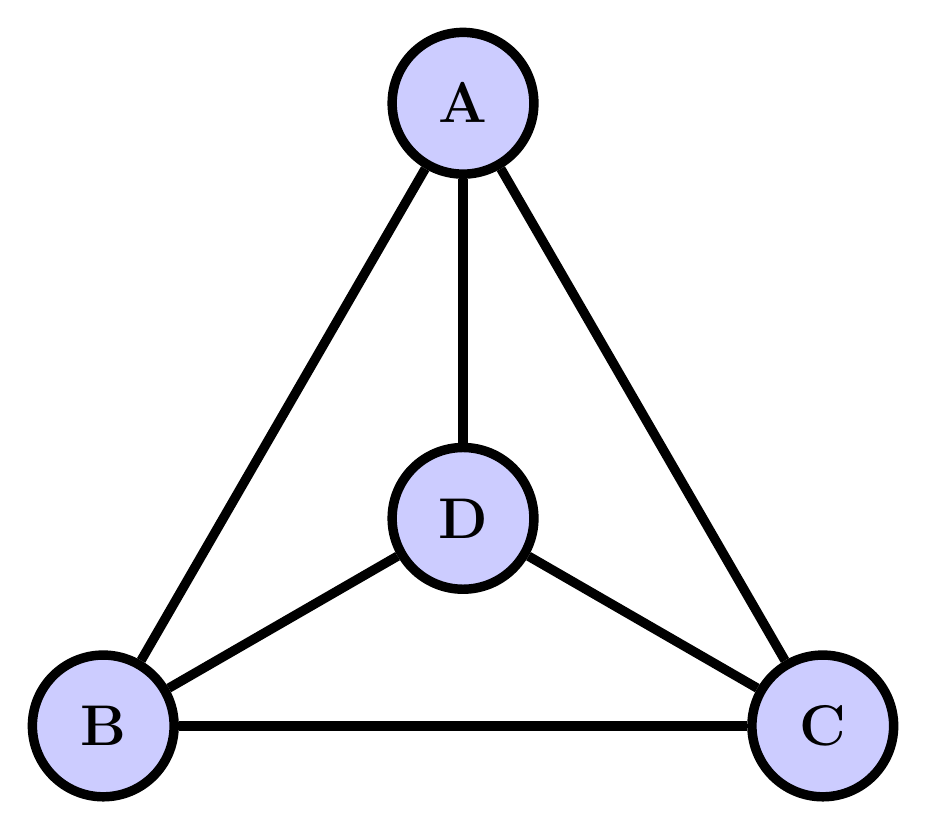
\begin{tikzpicture}
  \tikzset{
    mynode/.style={
      circle,
      draw=black,
      fill=blue!20,
      line width=1.2mm,
      minimum size=18mm,
      font=\bfseries\fontsize{20}{20}\selectfont,
      text centered
    }
  }

  \node[mynode] (A) at (0pt, 150pt) {A};
  \node[mynode] (B) at (-130pt, -75pt) {B};
  \node[mynode] (C) at (130pt, -75pt) {C};
  \node[mynode] (D) at (0pt, 0pt) {D};

  \draw[line width=1.2mm] (A) -- (B);
  \draw[line width=1.2mm] (B) -- (C);
  \draw[line width=1.2mm] (C) -- (A);
  \draw[line width=1.2mm] (D) -- (A);
  \draw[line width=1.2mm] (D) -- (B);
  \draw[line width=1.2mm] (D) -- (C);
\end{tikzpicture}%
}
\endgroup

}
  \caption{System of atoms bonded in a cage.}
\end{figure}

\begin{align}
    if\, q(\mathrm{A}|\mathrm{B}) &= 0 \nonumber \\
      & \implies q(\mathrm{A}) = q(\mathrm{A}|\mathrm{C}) + q(\mathrm{A}|\mathrm{D}) \nonumber \\
      & \implies q(\mathrm{B}) = q(\mathrm{B}|\mathrm{C}) + q(\mathrm{B}|\mathrm{D}) \nonumber \\
      & \implies q(\mathrm{B}|\mathrm{C}) = -q(\mathrm{C}|\mathrm{D}) \nonumber \\
      & \implies q(\mathrm{B}|\mathrm{D}) = -q(\mathrm{D}|\mathrm{A}) \nonumber \\
      & \implies q(\mathrm{B}|\mathrm{C}) + q(\mathrm{C}|\mathrm{D}) + q(\mathrm{D}|\mathrm{B}) = 0 \nonumber \\
      & \implies q(\mathrm{A}|\mathrm{C}) + q(\mathrm{C}|\mathrm{D}) + q(\mathrm{D}|\mathrm{A}) = 0 \nonumber \\
      & \implies q(\mathrm{B}) - q(\mathrm{B}|\mathrm{D}) + q(\mathrm{C}|\mathrm{D}) = 0 \nonumber \\
      & \implies q(\mathrm{B}) - q(\mathrm{B}|\mathrm{C}) + q(\mathrm{D}|\mathrm{A}) = 0 \nonumber \\
      & \implies q(\mathrm{B}|\mathrm{C}) - q(\mathrm{D}|\mathrm{A}) - q(\mathrm{B}|\mathrm{C}) + q(\mathrm{C}|\mathrm{D}) = 0 \nonumber \\
      & \implies q(\mathrm{D}|\mathrm{B}) + q(\mathrm{D}|\mathrm{A}) -q(\mathrm{B}|\mathrm{C})= 0 \nonumber \\
      & \implies q(\mathrm{B}|\mathrm{C}) + q(\mathrm{B}) - 2q(\mathrm{B}|\mathrm{C}) = 0 \nonumber \\
      & \implies q(\mathrm{B}) = q(\mathrm{B}|\mathrm{C}) \implies q(\mathrm{B}|\mathrm{D}) = 0 \nonumber \\
      & \implies q(\mathrm{B}|\mathrm{C}) = q(\mathrm{C}|\mathrm{D}) = q(\mathrm{B}) \nonumber \\
      & \therefore q(\mathrm{B}) = 0
\end{align}

